\documentclass[10pt]{beamer}

\usetheme{metropolis}
\usepackage{appendixnumberbeamer}

\usepackage{booktabs}
\usepackage[scale=2]{ccicons}

\usepackage{pgfplots}
\usepgfplotslibrary{dateplot}
\usepackage[]{algorithm2e}

\usepackage{xspace}
\newcommand{\themename}{\textbf{\textsc{metropolis}}\xspace}

\usepackage[utf8]{inputenc}
\usepackage[T1]{fontenc}

\usepackage{listings}
\usepackage{xcolor}
\lstdefinestyle{sharpc}{language=[Sharp]C, frame=lr, rul
	ecolor=\color{blue!80!black}}

\definecolor{bluevs}{RGB}{0,102,204}
\definecolor{greenvs}{RGB}{0,204,153}
\definecolor{pinkvs}{RGB}{255,0,102}
\definecolor{purplevs}{RGB}{102,0,204}

\title{Sistema de recomendação de regras para o Velocity}
\subtitle{API de Inteligência Computacional e Simulação}
\date{}
\author{Time Risco}
%\institute{Braspag}
\titlegraphic{\hfill
\includegraphics[height=1.5cm]{imgs/logo.png}}

\begin{document}
\maketitle

\begin{frame}{Sumário}
  \setbeamertemplate{section in toc}[sections numbered]
  \tableofcontents[hideallsubsections]
\end{frame}

\section{Introdução}

\begin{frame}[fragile]{Objetivos}
	\begin{itemize}
		\item Possibilitar que clientes Braspag testem combinações de regras do Velocity através de simulações com dados reais;
		\item Encontrar as melhores combinações de regras do Velocity para os clientes;
	\end{itemize}
\end{frame}

\section{Tecnologias}

\begin{frame}[fragile]{Benchmark C\# e Rust}
	\begin{center}
		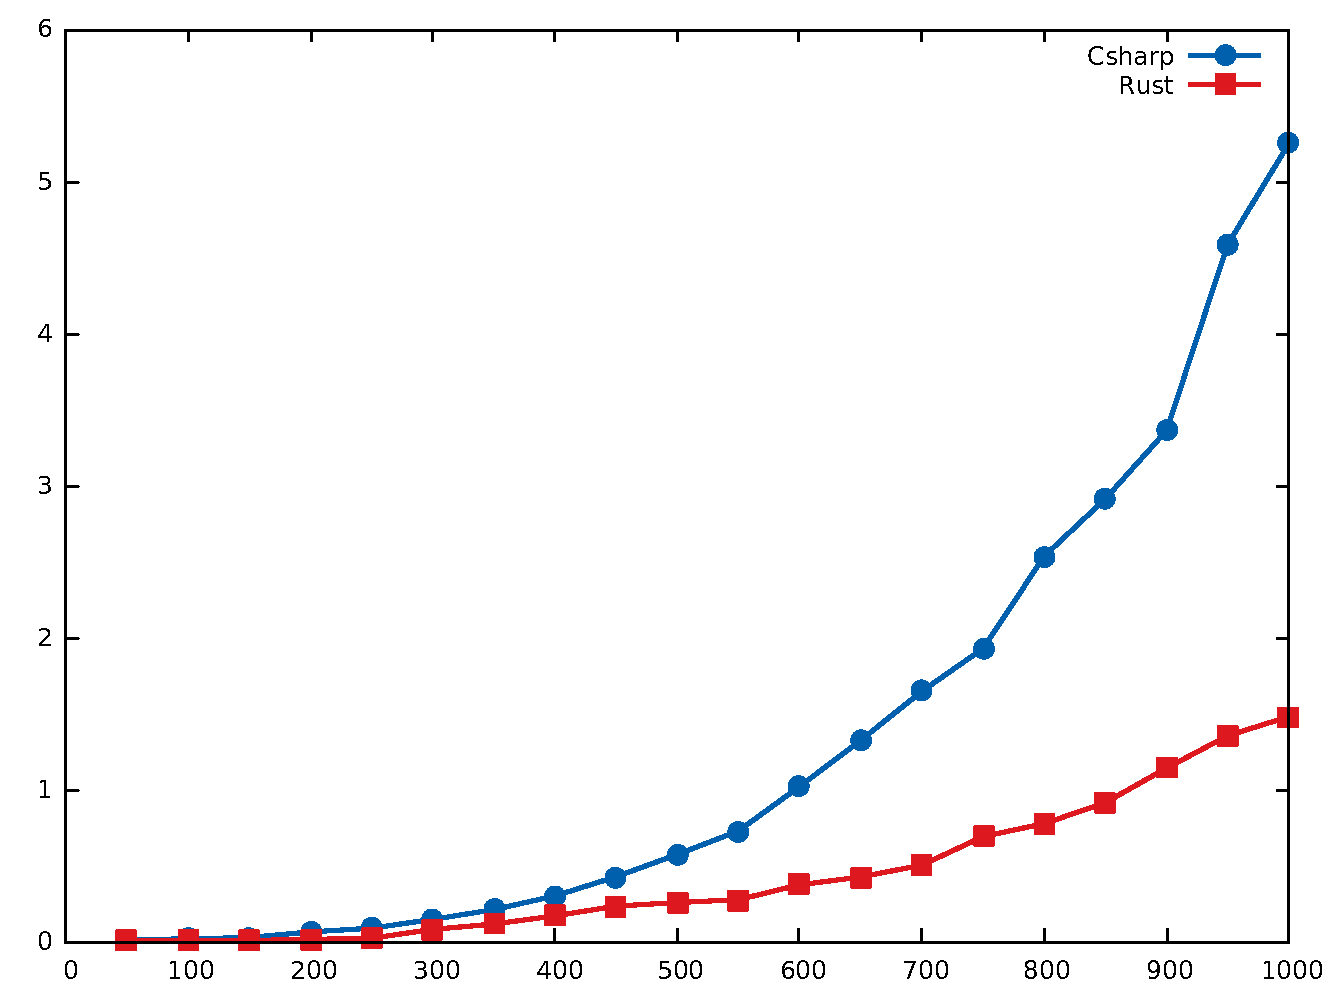
\includegraphics[scale=0.38]{imgs/graph.pdf}
	\end{center}
	\begin{itemize}
		\item Multiplicação de Matrizes NxN. Complexidade \textcolor{bluevs}{$O_{N \times N}(N^3)$};
	\end{itemize}
\end{frame}

\begin{frame}[fragile]{Complexidade de Simulações do Velocity}
	\footnotesize
	\begin{algorithm}[H]
		\ForEach{\textcolor{greenvs}{transaction} \textbf{in} \textcolor{pinkvs}{transactions}}{
			
			\vspace{0.1cm}
			
			\ForEach{\textcolor{greenvs}{rule} \textbf{in} \textcolor{pinkvs}{rules}}{			
				
				\vspace{0.1cm}
					
				\eIf{\textcolor{bluevs}{IsInQuarentine}(\textcolor{greenvs}{transaction}.\textcolor{purplevs}{parameter})}{
					
					\vspace{0.1cm}
					
					\textcolor{bluevs}{Block}(\textcolor{greenvs}{transaction});
					
					\vspace{0.1cm}
					
					\If{\textcolor{bluevs}{ExtrapolatesRule}(\textcolor{greenvs}{transaction}.\textcolor{purplevs}{parameter})}{
						
						\vspace{0.1cm}
						
						\textcolor{bluevs}{UpdateQuarentine}(\textcolor{greenvs}{transaction}.\textcolor{purplevs}{parameter});
						
						\vspace{0.1cm}
						
					}
					
				}{
					\vspace{0.1cm}
					
					\If{\textcolor{bluevs}{ExtrapolatesRule}(\textcolor{greenvs}{transaction}.\textcolor{purplevs}{parameter})}{
						
						\vspace{0.1cm}
						
						\textcolor{bluevs}{Block}(\textcolor{greenvs}{transaction});
						
						\textcolor{bluevs}{UpdateQuarentine}(\textcolor{greenvs}{transaction}.\textcolor{purplevs}{parameter});
						
						\vspace{0.1cm}
					}
				}
			}
		}
	\end{algorithm}
	\normalsize
	\begin{itemize}
		\item Algoritmo do Velocity. Complexidade \textcolor{bluevs}{$O_V(Transactions\hspace{0.1cm}x\hspace{0.1cm}Rules\hspace{0.1cm}x\hspace{0.1cm}Hits\hspace{0.1cm}x\hspace{0.1cm}Quarentine\hspace{0.1cm}x\hspace{0.1cm}R$)};
	\end{itemize}
\end{frame}

\begin{frame}[fragile]{Complexidade de Simulações do Velocity em Rust}	
	\begin{block}{Multiplicar Matrizes de 1000x1000}
		\textcolor{purplevs}{$O_{N \times N}(1000^3)$} -> \textcolor{purplevs}{Aproximadamente 1.4 segundos}
	\end{block}	
	
	\vspace{0.5cm}
	
	\begin{block}{140000 transações, 10 regras de 10 minutos, quarentena de 1 dia}
		\textcolor{purplevs}{$O_V(140000\hspace{0.1cm}x\hspace{0.1cm}10\hspace{0.1cm}x\hspace{0.1cm}10\hspace{0.1cm}x\hspace{0.1cm}140000\hspace{0.1cm}x\hspace{0.1cm}R)$} -> \textcolor{purplevs}{Aproximadamente 1.4 segundos}
	\end{block}	
	
	
	\vspace{0.5cm}
	
	\begin{block}{140000 transações, 10 regras de 7 dias, quarentena de 1 dia}
		\textcolor{purplevs}{$O_V(140000\hspace{0.1cm}x\hspace{0.1cm}10\hspace{0.1cm}x\hspace{0.1cm}10\hspace{0.1cm}x\hspace{0.1cm}140000\hspace{0.1cm}x\hspace{0.1cm}R)$} -> \textcolor{purplevs}{ Aproximadamente 6 minutos}
	\end{block}		
\end{frame}

\begin{frame}[fragile]{Complexidade de Simulações do Velocity em C\#}	
	\begin{block}{Multiplicar Matrizes de 1000x1000}
		\textcolor{purplevs}{$O_{N \times N}(1000^3)$} -> \textcolor{purplevs}{Aproximadamente 5.2 segundos}
	\end{block}	
	
	\vspace{0.5cm}
	
	\begin{block}{140000 transações, 10 regras de 10 minutos, quarentena de 1 dia}
		\textcolor{bluevs}{$O_V(140000\hspace{0.1cm}x\hspace{0.1cm}10\hspace{0.1cm}x\hspace{0.1cm}10\hspace{0.1cm}x\hspace{0.1cm}140000\hspace{0.1cm}x\hspace{0.1cm}R)$} -> \textcolor{bluevs}{Aproximadamente 5.2 segundos}
	\end{block}	
	
	
	\vspace{0.5cm}
	
	\begin{block}{140000 transações, 10 regras de 7 dias, quarentena de 1 dia}
		\textcolor{bluevs}{$O_V(140000\hspace{0.1cm}x\hspace{0.1cm}10\hspace{0.1cm}x\hspace{0.1cm}10\hspace{0.1cm}x\hspace{0.1cm}140000\hspace{0.1cm}x\hspace{0.1cm}R)$} -> \textcolor{bluevs}{No mínimo 22 minutos}
	\end{block}		
\end{frame}

\begin{frame}[fragile]{Complexidade de Simulações do Velocity Paralelo em Rust}	
	\begin{block}{140000 transações, 10 regras de 10 minutos, quarentena de 1 dia}
		\textcolor{purplevs}{$O_V(140000\hspace{0.1cm}x\hspace{0.1cm}10\hspace{0.1cm}x\hspace{0.1cm}10\hspace{0.1cm}x\hspace{0.1cm}140000\hspace{0.1cm}x\hspace{0.1cm}R)$} -> \textcolor{purplevs}{Aproximadamente 0.6 segundos}
	\end{block}	
	
	
	\vspace{0.5cm}
	
	\begin{block}{140000 transações, 10 regras de 7 dias, quarentena de 1 dia}
		\textcolor{purplevs}{$O_V(140000\hspace{0.1cm}x\hspace{0.1cm}10\hspace{0.1cm}x\hspace{0.1cm}10\hspace{0.1cm}x\hspace{0.1cm}140000\hspace{0.1cm}x\hspace{0.1cm}R)$} -> \textcolor{purplevs}{ Aproximadamente 3 minutos}
	\end{block}		
\end{frame}

\begin{frame}[standout]
  Obrigado
\end{frame}

\end{document}
